% Chapter 2

\chapter{Dynamic Modelling of TFAs} % Main chapter title

\label{Chapter2} % For referencing the chapter elsewhere, use \ref{Chapter3} 

\lhead{Chapter 2. \emph{Dynamic Modelling of TFAs}} % This is for the header on each page - perhaps a shortened title

%----------------------------------------------------------------------------------------

% \section{Literature Review}

In modern molecular biology the biological systems like cells are treated as a complex systems.
The usual conception of the complex system is a very large number of simple but identical elements 
interact to generate the complex behaviour. But the actual behaviour of biological systems are 
different from this conception. A vast number of functionally different and multifunctional 
group of elements act with each other selectively, perhaps nonlinearly to generate coherent 
instead of complex behaviour. Mostly, functions of biological systems depend on a combination of 
the network and specific elements involved. 

Development of molecular biology has discovered a large number of biological facts like sequencing 
genome, protein properties etc. But to explain the biological systems behaviour only these are not sufficient.
Study of cell tissues, organs, organisms etc. are also the systems of components to consider and 
their specific interaction which is defined by the evolution could be more supportive to reach the 
prime goal of biology. Though advancement in more accurate quantitative experimental approach will 
continue, but the detail functional insights of biological systems may not give the exact results 
from purely intuitive basis due to the intrinsic complexity of biological systems. A proper 
combination of experimental and computational approaches is more likely to solve this problem.

In modern molecular biology the organisational and functional activity of gene regulatory network 
is a key experimental and computational challenge.

\section{Gene Expression Data for Genomics }
Living cells contains thousands of genes. These genes codes for one or more protein. Expression of 
these genes are regulated by many of these protein through a very complex regulatory pathway.
Usually this regulation occurred to accommodate the change of the environment, as well as through 
the cell cycle of the development process. %TODO
Gene expression is the process where information contains in the gene is used to synthesis a 
functional gene product. The genetic code stored in the DNA usually expressed or interpreted by 
gene expression which represents the  phenotype. 
These gene expression data are usually stored in DNA microarray or DNA chip which is also known as
biochip. 

\begin{figure}[b]
	\centering
		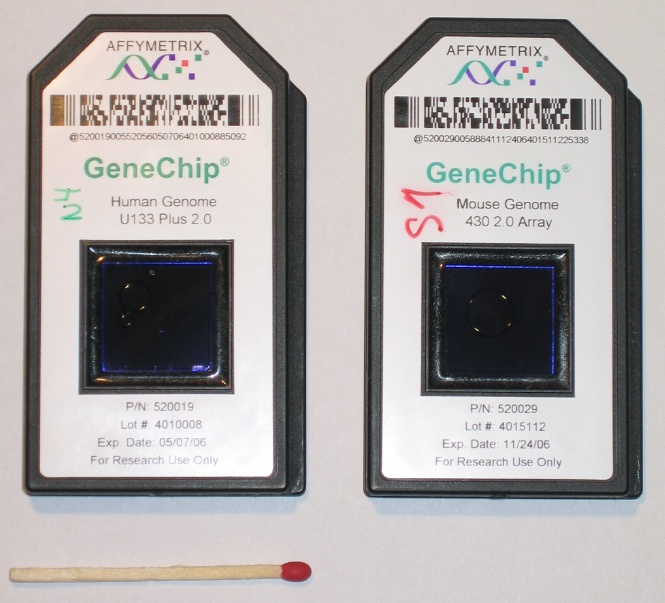
\includegraphics[width=.4\textwidth,keepaspectratio]{diagrams/Affymetrix-microarray.jpg}
		\rule{35em}{0.5pt}
	\caption{Gene Expression Data: Affymetrix Micro Array
	(Image courtesy Wikipedia. 
	\url{http://en.wikipedia.org/wiki/DNA_microarray})}
	\label{fig:Affymetrix-microarray}
\end{figure}
 
Figure \ref{fig:Affymetrix-microarray} shows two Affymetrix chips which contains DNA microarray. 
A match is shown at the bottom for the purpose of size reference of a microarray.
The solid-phase DNA macroarray is usually a collection of ordered microscopic spots called features.
Figure \ref{fig:Gene Expression Microarray} shows the schematic of the gene expression microarray data. 
On a typical Affymetrix microarray there are 6.5 million locations (represented by columns) with 
millions of identical DNA strands in every locations. Every strand construct with 25 probes or bases. 
The microarray is rinsed and washed with fluorescent stain. To accomplish a DNA test, two types of
samples are used one is controlled sample and another is test sample. 
After extracting mRNA from DNA, copied are made from mRNA by reverse transcription. 
Two different fluorescent tagged with cyanide are usually used to differentiate between controlled 
samples and test samples. In general, green is used for controlled copy and red for test copy. 
Then the tagged samples are washed on the microarray. 
DNA is analysed based on matching with the probes on the microarray.
A laser is used to glow the fluorescent molecules. After the hybridisation process
a green spot represents a hybridisation with the controlled targets only, a red spot indicates 
hybridisation with the test targets only, yellow represent hybridisation both with the controlled 
targets and test targets, and black represents hybridisation with the neither samples, i.e. 
no hybridisation. Over the last couple of decades these gene expression data became one of the key 
resource of the biologists to diagnose diseases and drug discovery, gene discovery and determining 
genetic variations, aligning and comparing genetic codes, biomerker development, forensic application, 
functional analysis and also in the field of computational biology.

\cite{Ong:2002} modelled the regulatory pathway in E.coli
from the time series gene expression microarray data by modelling causality, feedback loops or 
hidden variables using a Dynamic Bayesian network and tried to gain the insight of regulatory pathway.
By analysing gene expression data \cite{Friedman:2000} were the first to determine the properties 
of transcriptional program for Baker's yeast using a Bayesian network.

\begin{figure}[t]
	\centering
		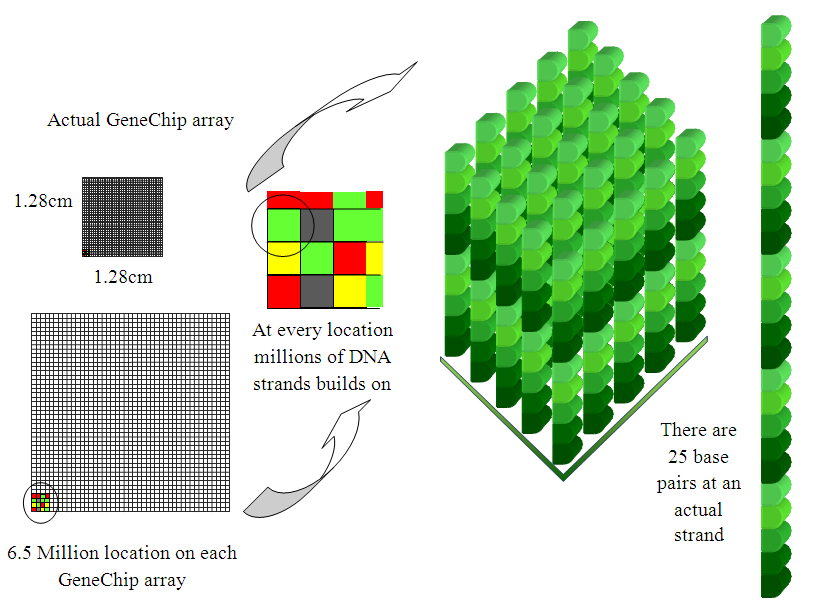
\includegraphics[width=\textwidth,keepaspectratio]{diagrams/GeneExpressionMicroarray.PNG}
		\rule{35em}{0.5pt}
	\caption{Gene Expression Data: Affymetrix Micro Array}
	\label{fig:Gene Expression Microarray}
\end{figure}

Many of the recent studies already established 
the fact that the gene function of regulatory network depends on qualitative as well as 
quantitative aspects of the organisation of the network like high throughput data, including 
genomic sequence, expression profiles and transcription factor.

Among them one of the major challenges is to quantitative measurement and analysis of the 
mechanisms regulating mRNA transcription. Though using high throughput techniques it is 
comparatively easier to measure the output of transcription, but it is experimentally 
very complicated to measure the protein concentration levels of transcription factors and 
chemical affinity to the genes. Very often transcription factors are post-transcriptionally modified. 
So, the actual protein concentration levels and binding affinities could be an unreliable proxy 
of the mRNA expression levels of transcription factors (\cite{Sanguinetti:2006}).

Due to the advancement of the experimental technique lot of interest in recent years has been 
growing to infer information about regulatory activity from target genes. Now biologists can 
acquire the information about the structure of the transcriptional regulatory network.  
\cite{Lee:2002} determined the transcriptional regulatory network of yeast using 
chromatin immunoprecipitation(ChIP). They tried to figure out how yeast transcriptional regulators 
bind to promoter sequences across the genome. By calculating a confidence value (\textit{P} value)
and setting up specific threshold they considered the protein-DNA interactions and artificially
imposes a binding or not binding binary decision for each of the protein- DNA pair.

\section{Connectivity Information}
\cite{Xie:2005} used motif conservation information for higher organisms like human, dog, rat 
and mouse. For promoter analysis they considered a number of network motif 
(also known as transcription factor binding sites) and also some new motifs. These type of data termed as 
connectivity data \cite{Liao:2003} provide information about whether a certain transcription factor 
can bind the promoter region of a gene or not.

\section{Different models of TFAs}
In recent years most methods aim to infer a matrix of transcription factor activities (TFAs).
These TFAs are sum up in a single number at a certain experimental point to find 
the concentration of the transcription factor and its binding affinity to its target genes. 
Many of the researcher used different ways or algorithm to find out these TFAs. 
For example, \cite{Liao:2003} developed a data decomposition technique with dimension reduction and 
introduced ‘network component analysis’. This method takes account of the connectivity information 
by imposing algebraic constraints on the factors. They argued that classical statistical methods
such as principal component analysis and independent component analysis dose not consider the underlying 
network structure while computing low dimensional or hidden representation of a high-dimensional data sets 
like DNA microarray. 

\cite{Alter:2004} used a dimension reduction technique (SVD) to figure out TFAs and also the 
correlation between DNA replication initiation and RNA transcription during the yeast cell cycle. 
Using multivariate regression and backward variable selection 
to identify active transcription factors \cite{Gao:2004} targeted the same; 
\cite{Boulesteix:2005} used partial least squares (PLS) regression to infer the true TFAs 
from a combination of tRNA expression and DNA protein binding measurement. 
A major drawback of the above mentioned methods is that transcription factor activities do not 
hold any information regarding the strength of the regulators interactivity between the 
transcription factor and its different target genes. But it is expected that 
depending on the experimental conditions transcription factor activities can vary from gene to gene. 
Even it is also expected that different transcription factors may bind the same gene. 
In most of the cases, realistic information about the intervals may not be true as they were 
not based on fully probabilistic model. Moreover, false positives are always a problem for 
connectivity data, typically a large portion of Chip data suffers form it 
(\cite{Boulesteix:2005}). 
Furthermore, due to the various cellular process or changes in environmental conditions 
the structure of the regulatory network of the cell can change considerably.
Using regression-based methods it is difficult to track these changes. 
\cite{Nachman:2004} build a probabilistic model, using the basic framework of 
dynamic Bayesian networks using discrete random variables for protein concentrations 
and binding affinities. Though the model was more realistic but the computational complexity for 
genome-wide analysis can be expensive.

\section{Our Goal}
We will propose a dynamic model that extends the linear regression model of \cite{Liao:2003} 
and probabilistic model of \cite{Sanguinetti:2006} to model the distribution of each transcription 
factor acting on each gene. We will model the temporal changes in the gene-specific TFAs from 
time-series gene expression data using Gaussian process (a stochastic process whose consciousness comes from 
random values and where the random variables has a normal distribution and it is associated with every single 
point in a range of times or of space; \textit{Chapter 4} contains detail explanation). 
The covariance structure of the transcription factors will be shared among all genes. 
This approach will lead to a manageable parameter space and figure out useful information about the 
correlation of TFAs.

Initially to build our model we will use two datasets: the classical yeast cell cycle dataset of 
\cite{Spellman:1998} and the yeast metabolic cycle dataset of \cite{Tu:2005}. Both of the data 
sets were used to study the above mentioned models. So, these data will be a source of useful comparisons. 
In both cases the connectivity data will be Chip data (\cite{Lee:2002}; \cite{Harbison:2004}). 
Finally we will use the data set of Caenorhabditis elegans (\textit{C. elegans}) to obtain a deeper insight. 
\textit{C. elegans} was used to build the probabilistic functional gene network Network.


%----------------------------------------------------------------------------------------
%\section{{\color{red}TODO} Regulator density and network motif}
%\cite{Lee:2002} page 800